\documentclass[10pt,a4paper]{article}
\usepackage[utf8]{inputenc}
\usepackage[T1]{fontenc}
% \usepackage{titlesec}
\usepackage[compact]{titlesec}
\usepackage{graphicx}
\usepackage{xcolor}
\usepackage{tikz}
\usetikzlibrary{calc}
\usepackage{multicol}
\usepackage[percent]{overpic}
% \usepackage[none]{hyphenat}
\usepackage{longtable}
\usepackage{enumitem}
% \usepackage[demo]{graphicx}
% \usepackage{subfig}

\include{defs}

\usepackage{lipsum}
% \setlength{\parindent}{0in}
\setlength{\columnsep}{1cm}

%-------------------------------------

% Title Page
\title{Auckland's Port Relocation Solutions}
\author{Strategic Management Plan \newline\newline FC Consulting \newline Team 13}
% \date{\today}
%-------------------------------------

\begin{document}
\maketitle
\pagenumbering{roman}
%-------------------------------------

% Cover Sheet
\newpage
\thispagestyle{empty} % Removes header and footer
\tikz[overlay,remember picture] \node[opacity=1, at=(current page.center)] {
  \includegraphics[height=\paperheight,width=\paperwidth]{CoverSheet.pdf}}; % Use relevant image or pdf
\clearpage
%-------------------------------------

% Team Photo
\newpage
\section*{Team 13}
\tikz[remember picture,overlay] \node[opacity=1, yshift=-0.7cm, at=(current page.center)] {
  \includegraphics[height=0.85\paperheight,width=0.85\paperwidth]{teamPhoto.png}}; % Use relevant image or pdf
\clearpage
%-------------------------------------

\newpage
% \section*{Executive Summary}

% \refstepcounter{section}
%Add Image
\vspace*{-40mm} %Make image have no top margin
\begin{tikzpicture}
\node[inner sep=0pt] (x) at (0,0)
    {\hspace{-87mm}\includegraphics[width=\paperwidth]{sectionimage2.jpg}};
% \node[text width=10in] (Z) at (0,-1) {\color{white}\headingfont\Large\bfseries\uppercase{\hspace{-0.7cm}\thesection\hspace{0.5cm}Executive Summary}};
\node[text width=10in] (Z) at (0,-1) {\color{white}\headingfont\Large\bfseries\uppercase{\hspace{-0.7cm}Executive Summary}};
\end{tikzpicture}
%Modify TOC
% \addcontentsline{toc}{section}{\protect\numberline{\thesection}Executive Summary}
%   \sectionmark{Executive Summary}
\vspace{1.5mm}
% \\This report outlines the feasibility study for the potential relocation of the Ports of Auckland (PoA) in the North Island. The New Zealand cabinet has requested 303 Consulting to undertake this study. The PoA is under stress due to the significant freight capacity it continues to handle. With the port soon to be operating at full capacity, further study suggests that if nothing is done soon, the demand for freight goods will outweigh the amount of freight that can be imported and exported. This will not be economically viable for Auckland in the long term. 
% % \vspace{-4mm}
% \\ \newline This study considered the following stakeholder requirements:
% \begin{itemize}[noitemsep]
%     \vspace{-2mm}
%     \item Efficiently transporting freight with the use of existing road and rail networks
%     \item Reduce shipping traffic in PoA and congestion of traffic in wider Auckland
%     \item Determine overall financial feasibility for the proposed solution
%     \item Create economic expansion and opportunities in other areas of the North Island
% \end{itemize}
% Based on the following analysis, the recommended solution is to incrementally relocate shipping traffic to the Port of Tauranga (PoT), while reducing the amount of shipping traffic coming into Auckland. Re-scaling of the ports will take place over a 10 year period. It is proposed that these changes will begin in the year 2025. PoA will be reduced to roughly 20\% of its current operating traffic by the end of the 10 year period, while the PoT will be allowed to expand. 
% \\ \newline Several options were analysed using an iterative process. Unsuitable details were identified and eliminated, narrowing down potential courses of action. As a result, the solution incorporates ideas from a handful of initial options. We came to the conclusion that by maintaining the PoA and relocating some of the shipping traffic to PoT allows PoA to downsize over a number of years. This reduction in size will free up prime real estate on the waterfront, currently being occupied by the PoA and will ease on-road traffic congestion around the port in central Auckland.
% % \vspace{-4mm}
% \\ \newline The decision to build an entirely new port was vetoed as it was found that in order to make that a feasible alternative, significant infrastructure was required to be built in order to support freight traffic alongside the construction of an entirely new port. While this motion was initially attractive, topography surrounding potential sites (including Manukau, Muriwai and Kawakawa Bay) was complex and infrastructure to and from the port was going to be significant and costly. The solution we propose minimises the need to build infrastructure from scratch and utilises the potential for an increase in capacity of pre-existing ports. It also means that shipping routes are not going to be affected in any way as these routes already exist and are currently being used.
% % \vspace{-4mm}
% \\ \newline The infrastructure connecting the various ports will need to be upgraded, the project will make use of the Regional Rapid Rail plan, which will connect the PoA to Hamilton, and then will go to Tauranga. This takes advantage of further establishment of the “Golden Triangle” between Auckland, Hamilton and Tauranga. This will also fund the addition of a new rail from Hamilton to Tauranga and the expansion of the highway between Tauranga and state highway.
\\This report outlines the feasibility study for the potential relocation of the Port of Auckland (PoA). The New Zealand cabinet has requested 303 Consulting to undertake this study. The PoA is under stress due to freight handling nearing capacity. With the port soon to be operating at full capacity; studies suggest that if nothing is done soon the demand for freight will outweigh the amount of freight that can be imported and exported. This is not economically viable in the long term. 
\vspace{-4mm}
\\ \newline This study considered the following stakeholder requirements:
\begin{itemize}[noitemsep]
    \vspace{-2mm}
    \item Efficiently transporting freight with the use of existing road and rail networks
    \item Reduce shipping traffic in PoA and congestion of traffic in wider Auckland
    \item Determine overall financial feasibility for the proposed solution
    \item Create economic expansion and opportunities in other areas of the North Island
\end{itemize}
Based on the following analysis, the recommended solution is to incrementally relocate shipping traffic to the Port of Tauranga (PoT), while reducing the amount of shipping traffic coming into PoA. Re-scaling of the ports will take place over a ten year period. It is proposed that these changes will begin in the year 2025. PoA will be reduced to roughly 20\% of its current operating traffic by the end of this period, while the PoT will be allowed to expand. 
\vspace{-4mm}
\\\newline Several options were analysed using an iterative process. Unsuitable details were identified and eliminated, narrowing down potential options. Based on the analysis, the best solution is maintaining the PoA and relocating some of the shipping traffic to the PoT; allowing PoA to downsize over a number of years. This reduction in size will free up the prime real estate on the waterfront, currently being occupied by the PoA, and will ease on-road traffic congestion in Auckland CBD.
\vspace{-4mm}
\\\newline The decision to build an entirely new port was vetoed due to infeasibility. Significant infrastructure would be required to support freight traffic alongside the construction of an entirely new port. While this motion was initially attractive, topography surrounding potential sites (including Manukau, Muriwai and Kawakawa Bay) was complex and infrastructure to and from the port would be significant and exorbitant. The solution we propose minimises the need to build infrastructure and utilises PoT’s current capacity. 
\vspace{-4mm}
\\\newline The infrastructure connecting the various ports will need to be upgraded. Our proposed solution makes use of the Regional Rapid Rail plan, which will connect the Auckland to Hamilton and finish in Tauranga. This takes advantage of the Governments “Golden Triangle” initiative between Auckland, Hamilton and Tauranga, opening up the opportunity for increased funding for the \$15 billion project. This will also fund the addition of a new rail from Hamilton to Tauranga and the expansion of the main highways connecting to Tauranga.


\clearpage
%-------------------------------------

% Info Graphic
\newpage
\thispagestyle{empty} % Removes header and footer
\tikz[remember picture,overlay] \node[opacity=1, at=(current page.center)] {
  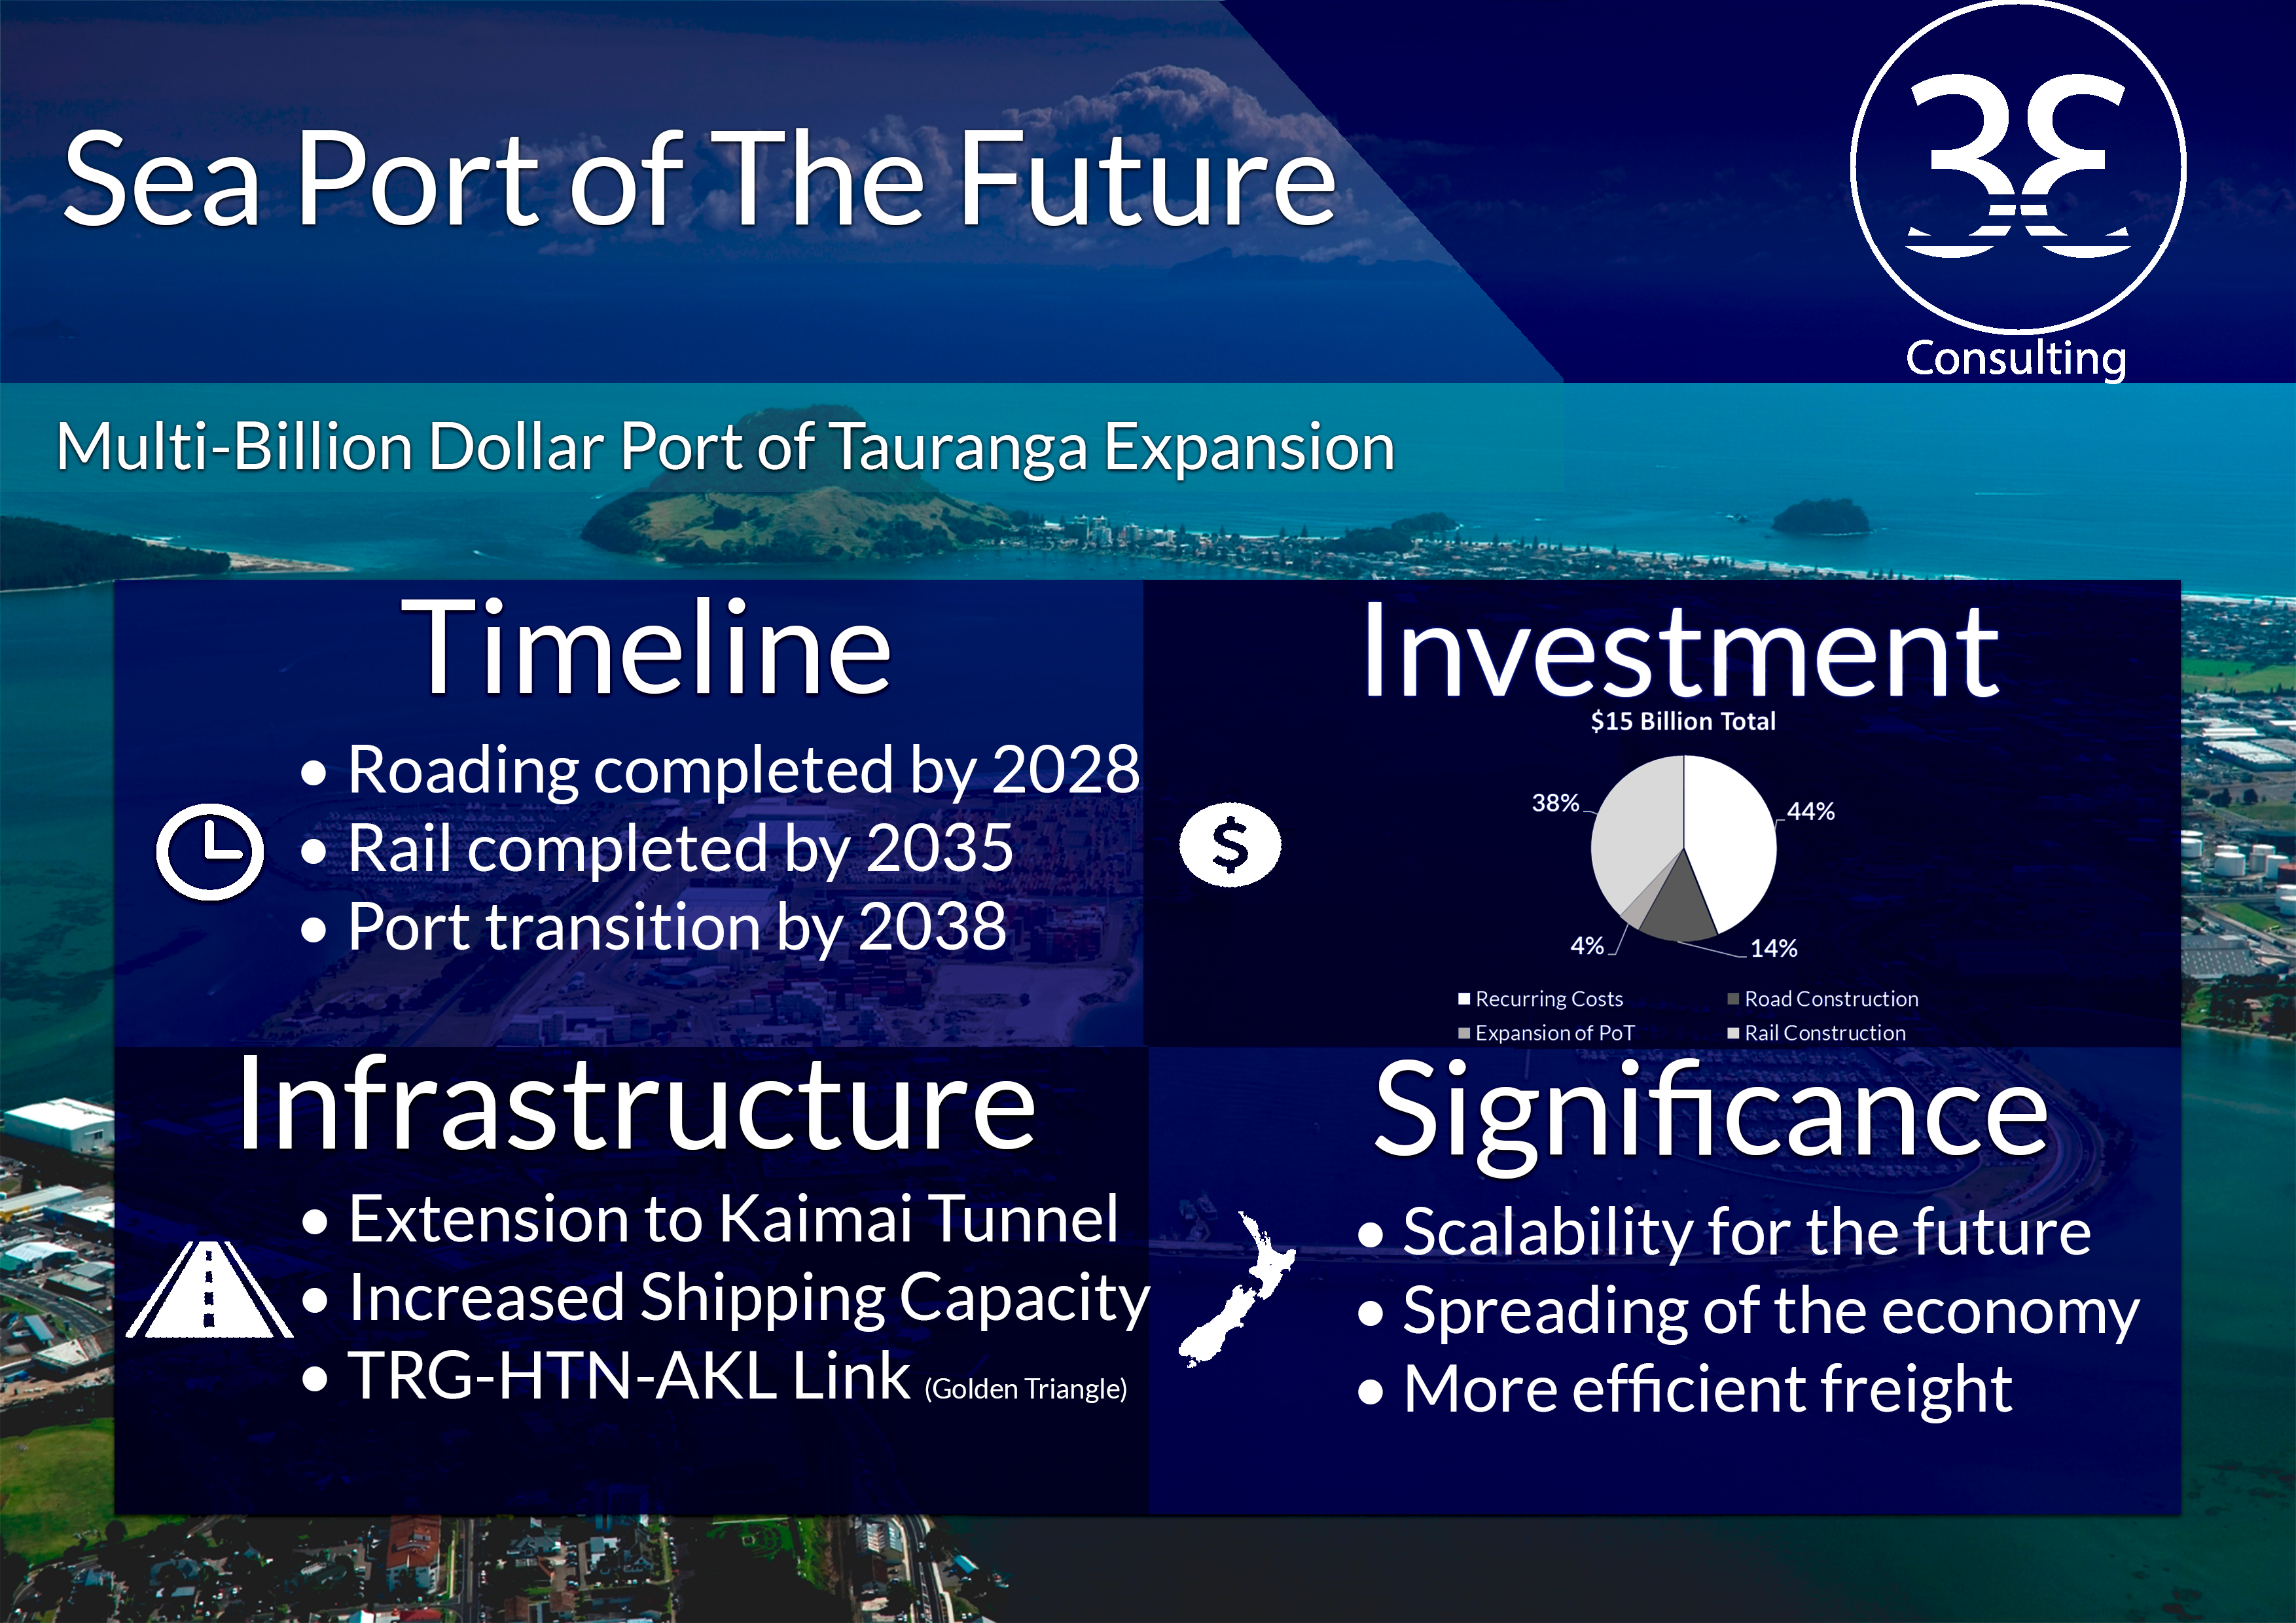
\includegraphics[height=\paperwidth,angle=90]{AtAGlance.png}}; % Use relevant image or pdf
\clearpage
%-------------------------------------

\newpage
\tableofcontents
\listoffigures
\listoftables
\clearpage
\pagenumbering{arabic}

% \include{defs.tex}

\newpage
\refstepcounter{section}
%Add Image
\vspace*{-40mm} %Make image have no top margin
\begin{tikzpicture}
\node[inner sep=0pt] (x) at (0,0)
    {\hspace{-87mm}\includegraphics[width=\paperwidth]{sectionimage3.jpg}};
\node[text width=10in] (Z) at (0,-1) {\color{white}\headingfont\Large\bfseries\uppercase{\hspace{-0.7cm}\thesection\hspace{0.5cm}Introduction}};
\end{tikzpicture}
%Modify TOC
\addcontentsline{toc}{section}{\protect\numberline{\thesection}Introduction}
  \sectionmark{Introduction}
\vspace{-2mm}

%Content
\subsection*{Background}
Auckland, known as the City of Sails, has one of the most illustrious views overlooking the Hauraki Gulf from downtown. From daily ferry services to luxury cruise ships, PoA has seen it all. As ships become larger, there is a concern regarding the infrastructure of the PoA is able to handle large volumes of goods imported and exported in the foreseeable future.
\\ Deputy Prime Minister of New Zealand, Hon Winston Peters, suggested during the election campaign that the PoA should be relocated to Whangarei which was agreed upon by the coalition government with Labour. As the demand for freight continues to grow, ports are required to develop their current facilities to cope with change. The PoA is soon to reach maximum operating capacity and will not be able to meet demand of freight. It currently occupies a lot of land which may provide alternative economic growth for Auckland. In addition, reducing container trucks near PoA will ease congestion of downtown traffic. 

\subsection*{Scope}
The scope for this project is to devise a plan for any long term potential relocation of the PoA. It is important to address any stakeholder conflicts the project may incur when in development. The overall cost of the project must be maintained within budget, whilst meeting health and safety, and environmental regulations. The relocation of the port is expected to occur over a 25-year period with at least 20\% still operating at PoA.

\subsection*{Goals}
This project is to determine whether a relocation of the POA is able to be implemented while meeting necessary stakeholder requirements and follow an economically feasible budget. To be successful the project must result in a more efficient and capable freight processing and distribution system which is able to handle the increase in freight quantity in the future.

\clearpage
\newpage

\refstepcounter{section}
%Add Image
\vspace*{-40mm} %Make image have no top margin
\begin{tikzpicture}
\node[inner sep=0pt] (x) at (0,0)
    {\hspace{-87mm}\includegraphics[width=\paperwidth]{sectionimage1.jpg}};
\node[text width=10in] (Z) at (0,-1) {\color{white}\headingfont\Large\bfseries\uppercase{\hspace{-0.7cm}\thesection\hspace{0.5cm}Stakeholder Analysis}};
\end{tikzpicture}
%Modify TOC
\addcontentsline{toc}{section}{\protect\numberline{\thesection}Stakeholder Analysis}
  \sectionmark{Stakeholder Analysis}
\vspace{-5mm}

%Content
% \section{Stakeholder Analysis}
    % \setlength{\columnsep}{0.5cm}
\begin{multicols}{2}
\subsection*{Auckland Council \& Residents} %of Auckland City, Whangarei, Tauranga}
    \textbf{The Auckland Council organisation as a whole is responsible for operation and service delivery, advising the governing body and local boards and carrying out their decisions. They represent the local Auckland residents. Residents include those who live in  the city and downtown areas that may be directly affected by construction on the waterfront. They are the consumers of shipped products}
    \\Auckland Council currently holds 100\% ownership of the Port of Auckland, receiving a net profit after tax as reported in 2017 of \$60.3 million per year. The Auckland Council is likely to be resistive to a relocation of the port outside of Auckland as removing freight removes a major source of revenue. Auckland already supports a population of 1.65 million and this number continues to rise at a rate of 1.9\% per annum. This growing population has growing demand and in turn, a larger volume of freight is needed to support this.
\subsection*{Central Government}
    \textbf{The New Zealand Central Government contains working groups that investigate the feasibility of projects and report directly to the Cabinet Office, influencing government decision making. They are interested in the continued economic growth of the country and will take into consideration factors in New Zealand’s revenue that influence this, namely tourism.}
    \\Alongside executive decision making power, the Central Government is assumed to provide significant funding and is likely to be supportive of the project if it is perceived to add value to the country and the government reputation. For tourism, Cruise ships docking in the PoA currently contribute an estimated \$204 million to the \$7.4 billion Auckland visitor economy. It is predicted by 2030 that this will rise to a \$470 million contribution. This increased tourism income will require more docking capacity for these cruise ships and less freight ship congestion in Auckland.
\subsection*{Transport Agencies}
    \textbf{Local government controlled agencies are responsible for developing possible transport solutions around New Zealand. Within this, KiwiRail is the largest rail transport operator in New Zealand. They are responsible for all rail operations in New Zealand. Their main aim will be to ensure the roads and/or railways are fit for purpose.}  
    \\ Responsible for any new roading and/or rail built in the case of a relocated port. Transport routes and frequency will have to change to accommodate for redistribution of freight. Transport agencies will not be significant contributors, however will be supportive if it does require any developments of the current road network.
\subsection*{Other City Councils}
    \textbf{Tauranga City Council, Northland City Council, and Whangarei District Council will meet the requirements of the locals by providing substantial development within their respective areas. }
    \\With regards to relocation of the Auckland port, other city councils will be significantly important and supportive. These councils would want to develop current infrastructure of the ports to compensate for the immediate future. These councils represent both the residents of their regions and their respective ports. This will provide more job opportunities for the different regions and with this, will be able to generate additional revenue. These job opportunities and revenue help to provide the growth needed to further develop any necessities required by the councils.
\subsection*{Port of Auckland Users}
    \textbf{Port Workers encompass everyone directly affected by the final solution. This includes any shipping company in Auckland and any current workers as they have to change their destination if there is reallocation. Moving and distributing freight via the Auckland Port will also be considered as Port users.}
    \\The Port of Auckland currently employs 500 direct jobs and they support approximately 187,000 jobs that facilitate the port proceedings. Reallocation of the Auckland port will result in redundancy of employees and a change in freight destination for shipping companies.  Some workers will be required to relocate with many unable to move. This will come at a great personal/financial cost for many of the workers.
\subsection*{Investors}
    \textbf{Investors provide feasibility for all projects around New Zealand. To cope with relocation of the port, they will be of high importance and will be supportive provided the relocated port can provide with a greater return of their investments.}
    \\The investors are companies, individuals, groups or organisations assumed to be providing funds for the project. They will expect a substantial return on investments.
    
% \subsection{Stakeholder 4}
% \lipsum[1-2]
% \subsection{Stakeholder 5}
% \lipsum[1]
\end{multicols}

\begin{wrapfigure}{l}{\linewidth}
\centering
\includegraphics[width=0.7\textwidth]{StakeholderMatrix.png}
\centering
\caption{Stakeholder Analysis Matrix}
\end{wrapfigure}


%Restore geometry 
% \restoregeometry
\clearpage
\newpage

\refstepcounter{section}
%Add Image
\vspace*{-40mm} %Make image have no top margin
\begin{tikzpicture}
\node[inner sep=0pt] (x) at (0,0)
    {\hspace{-87mm}\includegraphics[width=\paperwidth]{sectionimage2.jpg}};
\node[text width=10in] (Z) at (0,-1) {\color{white}\headingfont\Large\bfseries\uppercase{\hspace{-0.7cm}\thesection\hspace{0.5cm}Stakeholder Requirements}};
\end{tikzpicture}
%Modify TOC
\addcontentsline{toc}{section}{\protect\numberline{\thesection}Stakeholder Requirements}
  \sectionmark{Stakeholder Requirements}
\vspace{-5mm}
  
%Content
\begin{multicols}{2}
\subsection*{Efficient Freight Transport}
    \begin{flushleft}
        \textbf{Stakeholders: }\textit{Transport Agencies, Port Users}
    \end{flushleft}
    \vspace{-3mm}
    Allow freight to be distributed within the North Island more efficiently.
\subsection*{Projected Economic Value}
    \begin{flushleft}
        \textbf{Stakeholders: }\textit{Central Government, External Councils, Auckland Council}
    \end{flushleft}
    \vspace{-3mm}
    Solution should provide short and long term economic opportunities to the chosen region, and allow the economic status of the country to grow and improve. 
\subsection*{Reduce Traffic Congestion in Auckland}
    \begin{flushleft}
        \textbf{Stakeholders: }\textit{Auckland Council/Residents, Transport Agencies, External Supporting Councils}
    \end{flushleft}
    \vspace{-3mm}
    Improving efficiency for all road and rail users, both public and private. 
\subsection*{Environmental Impacts and Resource Efficiency}
    \begin{flushleft}
        \textbf{Stakeholders: }\textit{Central Government, External Supporting Councils, Auckland Council/Residents, Transport Agencies, Investors}
    \end{flushleft}
    \vspace{-3mm}
    Sustainable and efficient use of natural resources in such a way that environmental impacts are reduced. Natural capital should be used as efficiently as possible.
\subsection*{Ensuring Safety}
    \begin{flushleft}
        \textbf{Stakeholders: }\textit{Central government, External Supporting Councils, Auckland Council, Transport Agencies, Investors}
    \end{flushleft}
    \vspace{-3mm}
    The devised solution must ensure paramount safety of involved parties at all stages of the project. 
\subsection*{Transparency}
    \begin{flushleft}
        \textbf{Stakeholders: }\textit{Central Government, External Supporting Councils, Auckland Council/Residents, Transport Agencies, Investors, Port users}
    \end{flushleft}
    \vspace{-3mm}
    Ensuring there is clear, effective and constant communication between all concerned parties, the government and the general public.
\subsection*{Economic Feasibility}
    \begin{flushleft}
        \textbf{Stakeholders: }\textit{Transport Agencies, Auckland Council, Central Government, External Supporting Councils, Investors}
    \end{flushleft}
    \vspace{-3mm}
    Ensure the project costs falls within the required budget and completion occurs within an appropriate time frame.
\subsection*{Public Approval}
    \begin{flushleft}
        \textbf{Stakeholders: }\textit{Auckland Council/Residents, External Supporting Councils, Investors}
    \end{flushleft}
    \vspace{-3mm}
    Taxpayers must not oppose how their money is being utilised during development.
    
\end{multicols}    


\clearpage
\newpage
\refstepcounter{section}
%Add Image
\vspace*{-40mm} %Make image have no top margin
\begin{tikzpicture}
\node[inner sep=0pt] (x) at (0,0)
    {\hspace{-87mm}\includegraphics[width=\paperwidth]{sectionimage2.jpg}};
\node[text width=10in] (Z) at (0,-1) {\color{white}\headingfont\Large\bfseries\uppercase{\hspace{-0.7cm}\thesection\hspace{0.5cm}Options}};
\end{tikzpicture}
%Modify TOC
\addcontentsline{toc}{section}{\protect\numberline{\thesection}Options}
  \sectionmark{Options}
\vspace{-2mm}

%Content
\begin{multicols}{2}
\subsection*{Maintain Port of Auckland}
    \subsubsection*{Description}
    \textbf{The first option is to leave the PoA at its current location on reclaimed land in the Waitemata Harbour without development of the Port’s current geography.} \\The Port generates a yearly net profit after tax of approximately \$60 million and facilitates around 187000 jobs. It is comprised of 55ha of wharves and storage areas, the Port can support a 4000 TEU capacity.
    \\Referring to a study of the Port, the Auckland Council planning committee stated in October 2017 that the PoA will not be able to handle long-term freight and cruise demands. With no changes to current procedures, the port is expected to reach maximum capacity by 2030. However, leaving the Port ‘in-situ’ would continue to support the economic centre of freight in New Zealand, provide a best short term economic option in terms of feasibility and maintain the most efficient freight transport to reduce environmental impacts. This will ensure that there is no immediate impact on Auckland's economy and will avoid the need for initial capital investment by taxpayers and the government. It will also ensure that the current income from the port will remain in Auckland and there will be no fluctuation in land returns due to the reallocation of the land for other uses.

    \subsubsection*{Advantages}
    \begin{itemize}[noitemsep]
        \item []\textbf{Financial: }
        \item{If the port is moved, supporting ports will need extensive upgrades. Keeping the port will prevent massive short term costs and excessive revenue losses.}
        \item []\textbf{Natural: }
        \item{Natural resources will be used in upgrading infrastructure should the port be moved.}
        \item []\textbf{Human: }
        \item{Port workers and Auckland based shipping companies will continue to provide economic opportunities for the Auckland region.}
        \item []\textbf{Social: }
        \item{Keeping the port will maintain current jobs in Auckland and will prevent any relocated employees from having to re-settle elsewhere.}
    \end{itemize}
    \subsubsection*{Disadvantages}
    \begin{itemize}[noitemsep]
        \item []\textbf{Financial: }
        \item{Prevents waterfront being used for higher-tech, more profitable real estate (eg to Canary Wharf). Limits diversifying exports/imports in NZ.}
        \item{Restricts economic growth in other areas of NZ.}
        \item []\textbf{Natural: }
        \item{Increased congestion will produce high levels of air and noise pollution}
        \item []\textbf{Human: }
        \item{Prevents new jobs in the region of the new port.}
        \item []\textbf{Social: }
        \item{Congestion will remain significant, which will affect movement of freight in both Auckland and the rest NZ.}
    \end{itemize}



\subsection*{Relocate Port to Northport}

    \subsubsection*{Description}
    \textbf{The second option is to relocate the Port of Auckland and its freight traffic in its entirety to Northport in Marsden Point.}
    \\Northport has the potential to expand their docking length, dry goods storage and develop 180 ha of available industrial land. The draught capability of 13m allows for larger cargo ships, allowing for more cargo transported per litre of fuel consumed. Relocation to Northport will be able to support New Zealand’s increasing freight traffic while simultaneously reducing congestion in Auckland CBD. However, effectively relocating the Port of Auckland to Whangarei would require a major upgrade of the Northland transport system to efficiently distribute freight around the North Island. Currently, there exists a single track North Auckland Line (NAL) which provides freight services between Auckland and Whangarei twice every weekday. Shifting Auckland's freight traffic to aligns well with the current government's plans as the new Labour–NZ First coalition government announced that it would spend \$800 million total on rehabilitating the NAL.

    \subsubsection*{Advantages}
    \begin{itemize}[noitemsep]
        \item []\textbf{Financial: }
        \item{Immediate increase in local jobs available in Whangarei.}
        \item{Immediate decrease in marine traffic in the Auckland Region.}
        \item{Upgrades to the NAL are scheduled by the new coalition government, who could provide significant funding.}
        \item{Increased distribution of Wealth to poorer region (Northland)}
        \item{Constant income of leasing PoA real estate (tourism etc.)}
        \item{The significantly larger port size increases freight capacity.}
        \item{Improvements in the design life of the roads within Auckland. }
        
        
        \item []\textbf{Natural: }
        \item{Reduction in noise pollution in downtown Auckland.}
        \item{Reduced carbon emissions from less fuel usage in cargo ships.}
        
        
        \item []\textbf{Human: }
        \item{Improvement in the aesthetics of downtown Auckland}
        \item{Develop skills in the far north, increase population of working individuals.}
        \item{Decreased congestion in CBD improves the well-being of commuters}
        
        
        \item []\textbf{Social: }
        \item{Improves work ethic and hence socio-economic status of Northland populations.}
        \item{Urban development of the city of Whangarei.}
    \end{itemize}
    \subsubsection*{Disadvantages}
    \begin{itemize}[noitemsep]
        \item []\textbf{Financial: }
        \item{Significant costs of relocation (approx \$5 billion)}
        \item{Heavy cost associated with increasing road and/or capacity (currently 1 lane most of SH1).
        KiwiRail has estimated the cost of getting Northland’s rail network operating to the same standard as other regions as up to \$1 billion, and improving the rail link for freight through Auckland at another \$2 billion to \$3 billion}
        \item []\textbf{Natural: }
        \item{Destruction of habitat to increase roading and/or capacity (SH1)}
        \item []\textbf{Human: }
        \item{Relocation for workers in Port of Auckland}
        \item{Increased congestion between Northland and Auckland.}
        \item []\textbf{Social: }
        \item{Local iwi may be resistant to expansion of Marsden Point Port and Northland Transport network}
    \end{itemize}
 
\subsection*{Relocate Port to Tauranga}
  
    \subsubsection*{Description}
    \textbf{Option 3 is to relocate the PoA and its freight traffic in its entirety to the Port of Tauranga, the most efficient operating port in New Zealand.}
    \\Port of Tauranga currently has two sections in operation at Sulphur Point and Mount Maunganui. With an overall storage capacity available of 22000$m^2$ and with backup land capacity of 90 hectares available, the Port has capacity to grow and develop to meet New Zealand’s future freight demands. The water draught depth of 13.2m, allows the port of Tauranga to accommodate larger ships than the port of Auckland. This reduces the fuel consumption per container shipped. 
    \\The PoT is situated within the ‘Golden Triangle’, bound by Tauranga, Auckland and Hamilton, making it an ideal location for economic growth and distribution of wealth. However, relocation of PoA to Tauranga will require a significant transport infrastructure upgrade of current freight rail network between Auckland and Tauranga. This is to be able to distribute freight efficiently around the North Island and support increased freight traffic capacities from the redirected Auckland freight.  Rail development aligns with the government's plan to update the infrastructure within the ‘golden triangle’ in their Regional Rapid Rail plan.

   \subsubsection*{Advantages}
    \begin{itemize}[noitemsep]
        \item []\textbf{Financial: }
        \item{Tauranga would benefit from the increase in freight traffic from Auckland}
        \item{There's a existing port so one wouldn't have to be built from scratch}
        \item{Pre-existing infrastructure means you wouldn't need to build brand new lines to transport freight}
        \item []\textbf{Natural: }
        \item{Unprocessed industrial land can be developed to increase capacity}
        \item{Reclaimed land previously used for freight can be reallocated for other uses in the CBD}
        \item{reduce shipping based pollution in Auckland harbour}
        \item{Reduction of noise pollution in Auckland CBD}
        \item []\textbf{Human: }
        \item{Increase job opportunities}
        \item{Removal of the PoA will ease traffic congestion}
        \item []\textbf{Social: }
        \item{Further urban development of Tauranga}
        \item{Introduces new areas for the public in the CBD}
        \item{Improves the aesthetic of downtown Auckland}
    \end{itemize}
    \subsubsection*{Disadvantages}
    \begin{itemize}[noitemsep]
        \item []\textbf{Financial: }
        \item{Auckland’s economy would suffer from the delay in shipping (as it is no longer in Auckland)}
        \item{Increased cost of freight between Auckland and Tauranga}
        \item []\textbf{Natural: }
        \item{Increase in ship traffic will contribute to local pollution in Tauranga}
        \item{Expansion of the port will result in the destruction of natural habitats and environments.}
        \item []\textbf{Human: }
        \item{Reduction in job opportunities}
        % \item []\textbf{Social: }
        % \item{Congestion will remain a significant issue, which will affect movement of freight in both the region and the rest of the country.}
    \end{itemize}

\subsection*{Relocate to both Northport \& Tauranga}
    \subsubsection*{Description}
    \textbf{Option 4 is to relocate the waterfront PoA to an inland port and distribute all freight traffic between the Port of Tauranga and Northport. PoA would remain as a cruise ship and ferry docking terminal.}
    \\The relocation enables reclamation of land previously used for the PoA areas to be developed in such a way that it promotes the growth of the region’s tourism revenue. Additionally, this development would also increase the job and upskilling opportunities for those in Northland and Tauranga regions allowing for long-term economic development and increased accessibility for these communities. With the population of Auckland increasing by 50,000 people per year, the demand for freight is higher than ever and cannot be handled by a single operating port. Thus, it is essential to develop ports outside the Auckland region to accommodate the North Island’s inexorable increase in freight traffic. 
    \\Currently, 70\% of imports into the PoA are destined for the Auckland region so effective transport between the centres would be important in maintaining freighting efficiency. However, extensive upgrades to the road and rail network creates exorbitant capital expenses that may be unrealistic. 


    \subsubsection*{Advantages}
    \begin{itemize}[noitemsep]
        \item []\textbf{Financial: }
        \item{Increase in cash flow in Whangarei and Tauranga}
        \item{Population increase in such developing areas.}
        \item []\textbf{Natural: }
        \item{Reduced traffic congestion in Auckland}
        \item{Use of trains to reduce pollution (e.g electric trains)}
        \item []\textbf{Human: }
        \item{Immediate increase in job opportunities}
        \item{Develop skills in Northland and Tauranga}
        \item []\textbf{Social: }
        \item{Use of the waterfront area as a purely as a ‘community’ destination.}
    \end{itemize}
    \subsubsection*{Disadvantages}
    \begin{itemize}[noitemsep]
        \item []\textbf{Financial: }
        \item{The development of rail and road requires large initial investment}
        \item{Requires a large initial investment to establish the increased freight traffic at both ports.}
        \item []\textbf{Natural: }
        \item{Increase in shipping traffic in both harbours}
        \item{Increase in pollution}
        \item []\textbf{Human: }
        \item{Loss of port based jobs in Auckland}
        \item{Lack of these industrial skills in the Auckland region}
        \item []\textbf{Social: }
        \item{Local Iwi at Marsden Point may prevent development of the port and or cause problems in the future with ownership/management}
    \end{itemize}

\subsection*
{Other Ports in Auckland}
    \subsubsection*{Manukau Harbour}
    
        \textbf{Advantages: }{Frees up CBD area, low capital costs as naturally deep}
        \\\textbf{Disadvantages: }{West side(inconvenient), will require constant dredging, a decent population already resides in this area so will not be welcomed at all. Possible conflicts in regards to Mana Whenua and Treaty of Waitangi. Requires a major shift in shipping patterns}
    
    \subsubsection*{Kawakawa Bay}
        \textbf{Advantages: }{Deep water, large draught capacity and requires smaller change in shipping patterns.}
        \\\textbf{Disadvantages: }{Hunua ranges between Kawakawa and Auckland. As there is no existing port there, it must be built from the ground up. Surrounding infrastructure must also be constructed, adding to the overall cost.}
     
    \subsubsection*{Firth of Thames}
        \textbf{Disadvantages: }{Raises environmental, cultural and social issues. Ie: Very nature oriented area of NZ.Large scale reclamation required}
    
    \subsubsection*{Puhinui}
        {\textbf{Advantages: }Highest ranked on their NPV and CBA analysis. Lower capital cost compared to Firth of Thames. Smaller carbon footprint than the currently expanding POA}
        {\\\textbf{Disadvantages: }Will require strict legislations and practices to reduce environmental impacts. Dredging a lot. Future settlements may experience decreased water quality}
    
    \subsubsection*{Muriwai}
        \textbf{Advantages: }{Similar capital costs to making a new port in Firth of Thames.}
        \\\textbf{Disadvantages: }{Far from industrial centres. Further North/West than Manukau. Massive surf and rough weather present difficulties to docking and safety - coastline is exposed to weather from Tasman sea. Terrain inland is full of hills and narrow roads, very difficult to move freight through. Environmental pressure from locals - Large native gannet colony at Muriwai Recreational use of the beaches etc. will be significantly reduced.}  
    
\end{multicols} 

\clearpage
\newpage
\refstepcounter{section}
%Add Image
\vspace*{-40mm} %Make image have no top margin
\begin{tikzpicture}
\node[inner sep=0pt] (x) at (0,0)
    {\hspace{-87mm}\includegraphics[width=\paperwidth]{sectionimage3.jpg}};
\node[text width=10in] (Z) at (0,-1) {\color{white}\headingfont\Large\bfseries\uppercase{\hspace{-0.7cm}\thesection\hspace{0.5cm}Recycling Process}};
\end{tikzpicture}
%Modify TOC
\addcontentsline{toc}{section}{\protect\numberline{\thesection}Recycling Process}
  \sectionmark{Recycling Process}
\vspace{-2mm}


\subsection*{Recycling Diagram}
\begin{wrapfigure}{l}{\linewidth}
\centering
\includegraphics[width=0.9\textwidth]{RecylingDiagram.png}
\centering
\caption{Diagram of Recycling Process}
\end{wrapfigure}

\clearpage
\newpage
\refstepcounter{section}
%Add Image
\vspace*{-40mm} %Make image have no top margin
\begin{tikzpicture}
\node[inner sep=0pt] (x) at (0,0)
    {\hspace{-87mm}\includegraphics[width=\paperwidth]{sectionimage1.jpg}};
\node[text width=10in] (Z) at (0,-1) {\color{white}\headingfont\Large\bfseries\uppercase{\hspace{-0.7cm}\thesection\hspace{0.5cm}Best Fit Option}};
\end{tikzpicture}
%Modify TOC
\addcontentsline{toc}{section}{\protect\numberline{\thesection}Best Fit Option}
  \sectionmark{Best Fit Option}

\subsection*{Initial Best-fit Solution}
Following extensive research into possible Port relocation options, a M.A.R.T analysis was conducted to determine the viability of each option with consideration of the stakeholder requirements. This looked to analyse economic, environmental and societal aspects as well as the overall feasibility of the option. Each of these aspects were considered in terms of the key stakeholder requirements and weighted according to importance to help determine the best fit solution. Any underdeveloped areas were further iterated to establish a final solution that best fit the requirements and aims of the project. 
\\Out of the four considered options, keeping the Port of Auckland as is and the relocation of the Port of Auckland to Tauranga were determined to be the top two solutions closest to meeting the decided requirements. From the M.A.R.T analysis, it was clear relocating to Tauranga was the best fit option, this is especially prevalent when considering the points below:
\begin{itemize}[noitemsep]
    \vspace{-2mm}
    \item PoA would eventually need to expand and anticipate the need for change to allow for a smooth transition to better meet the public's approval (people want the waterfront area used for purposes other than freight).
    \item Redistributions of population densities and development of different regional areas
    \item Reduction of traffic congestion in Auckland.
    \item Tauranga is not at capacity yet and has potential to grow.
\end{itemize}
\subsection*{Justification}
Keeping the PoA in Auckland would see it heavily restricted in its future developments and it cannot solely maintain the predicted freight capacity that New Zealand hopes to support. Current congestion in the CBD reduces efficiency significantly and delaying the redistributions of freight traffic will come at a higher capital cost in the long term. 
\\The sole movement of freight traffic to Whangarei is not supported by a reliable transport network. The NAL is showing significant signs of wear and does not have the capacity to move the required volume of freight from Whangarei to Auckland. The costs of refurbishing and expanding the line would not justify the economic benefit of moving the PoA to Northland. 
\\Relocating the port hubs to both Port of Tauranga and Northport would require the upgrade of transport networks in both northbound and southbound directions to Whangarei and Tauranga respectively inducing heavy and unrealistic capital costs outweighing any social and economic benefits provided by the distribution of wealth.
\\In the first analysis, a relocation of the Port of Auckland to Tauranga proved to satisfy most of the Stakeholder Requirements. It reduced traffic congestion within Auckland and allowed for freight to be distributed efficiently around the North Island as Tauranga is located within the ‘Golden Triangle’. This proved to be more economically feasible in comparison to relocating the Port to Whangarei or a combination and also provided the best economic value and growth for the North Island. However, when the option was compared to the original Stakeholder Requirements, the complete relocation of the Port to Tauranga contained risks and options needed to be recycled to iterate for a better solution.
\subsection*{Optioneering}
Despite the Port of Tauranga being considered as the ‘least-worst’ of the four initial option, when compared to the project and stakeholder requirements, it was identified that the PoT alone would not have sufficient capacity to accommodate for Auckland’s freight traffic alongside its own. Additionally, the current transport infrastructure between Hamilton and Tauranga does not allow for redundancy in the event of damage.
\subsection*{Development of a Secondary Port around the Auckland Region}
\subsubsection*{Relocate the Port to Kawakawa Bay}
While Kawakawa Bay has sufficient draught capacity, a relocation of the Port would require the construction of significant infrastructure to make freight transport feasible. The lack of major transport infrastructure would exert exorbitant capital costs on the project. The location of the port also raises important cultural, social and environmental issues.
\subsubsection*{Relocate Port to Manukau}
Manukau Harbour is located on the west side of New Zealand, away from current shipping routes, which may result in increased shipping costs and a decrease in efficiency. Manukau’s high population density also limits port expansion. The shifting sandbar makes entrance into the Harbour difficult and would require constant dredging. Because it is located on Maori land, legislations and consents would be required for the project to proceed. 
\subsection*{Best Fit Option}
Given this analysis, retaining approximately 20\% of the existing PoA is the most feasible option as it allows for gradual relocation and builds redundancy into the design. Given that a split distribution between the Auckland and Tauranga Ports is the best option, freight transport infrastructure needs to be considered.
\subsection*{Development of Rail Lines}
Links between Auckland, Hamilton and Tauranga, need to be developed to the standard that would be required to handle the predicted freight transport capacity. Enhancing the current rail is part of the Regional Rapid Rail (RRR) passenger and freight transport plan developed by Labour Government. Any new freight lines developed for the PoT would follow the construction schedule of the RRR plan to streamline fabrication. The upgrade of the East Coast Main Trunk to a double rail line would increase the rail freight capacity. Another benefit of having two rails is that the other serves as a safeguard from accidents such as slips which threaten rail closures. 
\subsection*{Development of Road}
The sheer volume of freight requires multiple modes of transport. Upgrading the two-lane-two-way road over the Kaimai Ranges to a four-lane-two-way road will provide an alternative freight route to the existing rail line. In the case of natural disasters such as earthquakes or landslides, roads can also be utilised as a viable alternative to rail.
\\\newline This recycling process was beneficial as it allowed for ‘stakeholder feedback’, and with each iteration, modifications were made that improved the solution’s overall functional capability and better satisfied the problem.



\subsection*{Revised Best Fit Solution}

After analysing previous options, and referring back to our stakeholder requirements, it was determined that the option of moving all of PoA’s freight traffic to PoT was not technically feasible or efficient in the long term. It was then decided over an iterative process that the best solution was to minimise the port of Auckland to 20\% over a period of 10 years and transfer the excess shipping traffic to the PoT. This best fit option includes the gradual expansion of the PoT to compensate for the increase in freight traffic and the upgrade of the East Coast Main Trunk between the Hamilton and Tauranga ports. The connecting state highways will also be upgraded to further aid in freight transport as well as covering the risk of natural disasters such as landslides, and their effect in blocking trade routes.

\begin{figure}
\centering
\includegraphics[width=0.9\textwidth]{mart1.png}
\centering
\caption{MART Analysis}
\end{figure}
\begin{figure}
\centering
\includegraphics[width=0.7\textwidth]{ProjectFunding.png}
\centering
\caption{Project Funding}
\end{figure}


\clearpage
\newpage
\refstepcounter{section}
%Add Image
\vspace*{-40mm} %Make image have no top margin
\begin{tikzpicture}
\node[inner sep=0pt] (x) at (0,0)
    {\hspace{-87mm}\includegraphics[width=\paperwidth]{sectionimage3.jpg}};
\node[text width=10in] (Z) at (0,-1) {\color{white}\headingfont\Large\bfseries\uppercase{\hspace{-0.7cm}\thesection\hspace{0.5cm}Implementation}};
\end{tikzpicture}
%Modify TOC
\addcontentsline{toc}{section}{\protect\numberline{\thesection}Implementation}
  \sectionmark{Implementation}




\subsection*{PHASE 1 - Planning of Project}
Planning of construction will begin in 2020 and last approximately five years. Phase I involves identifying the required equipment, workforce, materials, and other resources needed to complete the project. The project includes the expansion of Port of Tauranga (PoT), and rail and road development from Auckland to Tauranga via Hamilton.

\subsection*{PHASE 2 - Expansion of PoT and Construction of Road and Rail}
By 2025, planning will be complete, and construction will begin. The project will involve three sub-projects in total; the initial expansion of the PoT, lane additions on State Highway 29 (SH29), and the construction of a new railway track between Hamilton and Tauranga, including a new Kaimai Ranges tunnel. 
\\To facilitate the partial transition of freight from PoA to PoT, the capacity of the road and rail needs to be increased. State Highway 1 (SH1) to SH29 is the proposed route for trucks to transport freight between Tauranga and Auckland. SH1 is currently a four-lane-two-way highway while SH29 is only a two-lane-two way road. It is proposed to upgrade SH29 to a four-lane-two-way road over a three-year timeframe. The first expansion of the PoT occurs in conjunction with highway development. 
\\The decrease in freight at PoA will vacate prime real estate on the waterfront. Leasing real estate will generate revenue to fund the construction costs of both the SH29 and railway upgrade from Tauranga to Hamilton. Road upgrades have a smaller capital investment than the rail line construction, \$2.04 billion as opposed to \$5.62 billion. Refer to the CBA in the appendix for estimated costs.
During the upgrade of SH29 and the expansion of PoT, there will be an additional rail line constructed beside the East Coast Main Trunk Line, located between Claudelands and Tauranga. This additional line improves freight transport efficiency and introduces redundancy as a safety factor. A major cost to this additional rail line will be the second tunnel through the Kaimai Ranges. This will need to be done as the existing tunnel does not have the capacity to facilitate another rail line. 


\subsection*{PHASE 3 - Begin Incremental Freight Transition}
By 2028, the PoT initial expansion and the SH29 lane addition will be complete. The transition of freight from PoA to PoT will commence, with the 8\% annual freight transition beginning in 2028. This transition will continue for ten years, terminating in 2038, when 80\% of the original total freight of PoA, is transitioned to PoT. 
\\After the second year of transitioning freight, there will be 16\% less freight handled at PoA, which is assumed for this analysis to proportionally vacate 16\% of PoA rest estate on the waterfront, this will not be a realistic expectation. This real estate can then be leased for just over \$1 billion, a partial sum of this will be put back into the project. This leasing cycle can continue in two-year increments during the freight transition phase. 

Refer to CBA in Appendices for future cash flows up until the transition terminates and PoA is at 20\% capacity (year 2035).

\subsection*{PHASE 4 - Secondary PoT Expansion Commences}
The second expansion commences in 2035 and terminates in 2038 to cater for the remaining freight from PoA as rail is now fully developed. By 2038, 80\% of Auckland freight will have been transitioned to the PoT.

\subsection*{PHASE 5 - Performance Assessment}
With the completion of construction and expansions, past statistics and data on pollution, recurring costs, traffic congestion, and other factors will be used to estimate whether or not the project will remain successful in the future.
\\Delays or Disruptions:
To account for delays or disruptions, in our analysis of the NPV, we extended the project timeline to be completed in 2044.

\subsection*{Economic and Financial Analysis}
The implementation of the project will have a total cost of approximately \$15 billion. The initial cost for the first two years of this project is approximately \$4 billion. The revenue we receive from both the Port of Auckland and the Port of Tauranga, will be approximately \$1 billion. The remaining \$3 billion will be evenly distributed and invested by the Central Government and the Public-Private Partnership. This is an estimation, and is dependant on many factors. Investments will be made continuously throughout the ten years of construction with another \$350 million investment in 2035 to expand the port of Tauranga.
\\The largest area of expenditure for our project, is the operating costs from the rail and roading freight networks. Over the 25-year scope of our project, the calculated estimation of freight transport operating costs, is \$6.55 billion total. This accounts for 44\% of the total costs of the project. This is illustrated in the pie graph, and the other costs of the project are compared.

\subsection*{Cost Benefit Analysis}
    \subsubsection*{Financial Capital}
        \begin{itemize}[noitemsep]
            \item[] \textbf{Capital Cost}
            \item Road Expansion  -  \$2.04 Billion
            \item Rail Construction - \$5.6 Billion
            \item Port Expansion - \$700 million
            \item[] \textbf{Benefit}
            \item Port of Auckland \& Net Profit \$206 million PA with a growth rate of 8\%
            \item Benefit from Land of Port of Auckland \$7.3 billion
        \end{itemize}
    \subsubsection*{Natural Capital}
        \begin{itemize}[noitemsep]
            \item First 10 years of transition, an additional 139,500 tonnes of CO2 will be emitted by the increase of freight trucks. The estimated emission of CO2 is approximated to 51.2 million litres. Assuming the CO2 emitted correlates to the amount of fuel consumed the estimate environmental cost for this project is evaluated to \$82 million PA.
            \item After the completion of the electric railway system CO2 emission will be reduced by 21 million litres. This equates to approximately \$33.6 million PA for environmental benefit.
        \end{itemize}
        Natural Capital is the stock of natural resources. We quantified the release of carbon emissions as an environmental cost in our NPV calculations. These figures are estimated as accurate as possible with the data we have.
    \subsubsection*{Social/Human Capital}
        \begin{itemize}[noitemsep]
            \item Due to reduced traffic congestion each person saves 20 minutes per day. Assuming the average wage is \$23/hr, and half the population of Auckland (700,000) travels by road, the benefit from reduced traffic congestion evaluates to approximately \$1.4 billion PA.
            \item Total salary in PoT is currently \$32 million. Expansion of PoT will increase employment by 80\% measuring to approximately \$57.6 million PA. 
            \item The project will increase Tauranga's GDP by 2\%. The predicted contribution to GDP by this project, will be approximately \$1.4 billion, evaluating to \$28 million PA contributed by the increase of port operations.
        \end{itemize}
        Human capital and Social capital is the value added by the wider community and personal wellbeing. The reduction of traffic congestion improves the quality of life for daily commuters in Auckland. The expansion of the port will also significantly increase local employment and cash flow, promoting regional and urban development in Tarunga.
        
\begin{figure}
\centering
\includegraphics[width=0.9\textwidth]{CostBySector.png}
\centering
\caption{Cost of Project by Sector}
\end{figure}

% \newpage
\begin{figure}
\centering
\includegraphics[width=0.9\textwidth]{implementationImage.png}
\centering
\caption{Current Rail Line/Road from Auckland to Tauranga}
\end{figure}

\begin{figure}
\centering
\includegraphics[width=0.9\textwidth]{Timeline.png}
\centering
\caption{Project Timeline}
\end{figure}

\clearpage
\newpage
\refstepcounter{section}
%Add Image
\vspace*{-40mm} %Make image have no top margin
\begin{tikzpicture}
\node[inner sep=0pt] (x) at (0,0)
    {\hspace{-87mm}\includegraphics[width=\paperwidth]{sectionimage2.jpg}};
\node[text width=10in] (Z) at (0,-1) {\color{white}\headingfont\Large\bfseries\uppercase{\hspace{-0.7cm}\thesection\hspace{0.5cm}Risks}};
\end{tikzpicture}
%Modify TOC
\addcontentsline{toc}{section}{\protect\numberline{\thesection}Risks}
  \sectionmark{Risks}
\vspace{-2mm}

%Content

\begin{wraptable}{l}{\linewidth}
\centering
\includegraphics[width=\textwidth]{risks.png}
\centering
\caption{Table of Potential Risks}
\end{wraptable}


% \begin{multicols}{2}
% \subsection*{Health and Safety Risks Associated with Construction of any Road or Rail Networks}
%     \textbf{Mitigation: }{Abide by any laws and regulations regarding health and safety, including safety in design.}

% \subsection*{Resistance of port workers to change way of life with a relocation of port may create public opposition}
%     \textbf{Mitigation: }{Ensure clear communication of project well in advance of scheduled relocation to allocate time for port workers to potentially relocate.}

% \subsection*{Resistance of Auckland Council to surrender a portion of the port capacity}
%     \textbf{Mitigation: }{Clearly outline the benefits associated with the development of tourism and urbanisation as an incentive for a partial relocation of the Port of Auckland.}

% \subsection*{Air pollution from the increased vehicle volumes on both road and rail}
%     \textbf{Mitigation: }{Any vehicle purchased for moving freight should ideally minimise fuel consumption and carbon dioxide emissions. Majority of freight is to be transported by rail rather than road.}
    
% \subsection*{Inadequate existing port infrastructure to support future development in Tauranga}
%     \textbf{Mitigation: }{Not covered in the report. Ruakura freight hub considered in design.}    
    
% \subsection*{Natural disaster risks which may cause temporary closure of freight transport route}
%     \textbf{Mitigation: }{Build redundancy into design by ensuring there are multiple pathways leading to the same destination.}

% \subsection*{Increased road traffic congestion over the         Kaimai ranges along the route linking Hamilton and          Tauranga}
%     \textbf{Mitigation: }{Perform lane expansion on both sides to make a two-way, two-lane road to accommodate for the increased traffic.}
   
% \subsection*{Insufficient revenue generated from leasing land during Phase III - Transition}
%     \textbf{Mitigation: }{Careful and thorough economic analysis needs to be undertaken to values land lease and a projected timeline for return on investment.}   
   
% \end{multicols} 


\clearpage
\newpage
\refstepcounter{section}
%Add Image
\vspace*{-40mm} %Make image have no top margin
\begin{tikzpicture}
\node[inner sep=0pt] (x) at (0,0)
    {\hspace{-87mm}\includegraphics[width=\paperwidth]{sectionimage3.jpg}};
\node[text width=10in] (Z) at (0,-1) {\color{white}\headingfont\Large\bfseries\uppercase{\hspace{-0.7cm}\thesection\hspace{0.5cm}Opportunities}};
\end{tikzpicture}
%Modify TOC
\addcontentsline{toc}{section}{\protect\numberline{\thesection}Opportunities}
  \sectionmark{Opportunities}
\vspace{-2mm}

\subsection*{Golden Triangle Development}

Development of the Regional Rapid Rail Project will help streamline the construction process and will provide additional support as the Golden Triangle develops. Highlighting the need for transportation development and efficiency, which may result in more funding in the future. 
\subsection*{Tourism}

With the reduction of pollution (noise and general) in the Hauraki Gulf and an increased capacity for cruise ships in the reduced PoA, it allows Auckland to accelerate its tourism while generating economic value with the development of the downtown area within Auckland CBD.
 
\subsection*{Population distribution}
The movement of the main Port Hub down to Tauranga promotes a chance in the current population distributions and relieve the pressures on Auckland City. The cleared areas on the Auckland waterfront during relocation will provide more downtown housing and parking and could lower Auckland house prices.  

\subsection*{Regional Development}
Tauranga has the ability to grow into a larger city. As it expands, the number of higher income jobs will increase. This increased wealth in the area will have the benefit of increasing quality of life for residents.

\subsection*{Traffic}
With enhancements in traffic control in both Auckland and Tauranga, the travel time within these twos cities will be reduced. Widening the roads will decrease traffic congestion for workers and hence increase productivity at the workplace. This will enhance the characteristics of the business and therefore help produce more revenue.


\clearpage
\newpage
\refstepcounter{section}
%Add Image
\vspace*{-40mm} %Make image have no top margin
\begin{tikzpicture}
\node[inner sep=0pt] (x) at (0,0)
    {\hspace{-87mm}\includegraphics[width=\paperwidth]{sectionimage4.jpg}};
\node[text width=10in] (Z) at (0,-1) {\color{white}\headingfont\Large\bfseries\uppercase{\hspace{-0.7cm}\thesection\hspace{0.5cm}Safety}};
\end{tikzpicture}
%Modify TOC
\addcontentsline{toc}{section}{\protect\numberline{\thesection}Safety}
  \sectionmark{Safety}
\vspace{-5mm}

\begin{multicols}{2}
\subsection*{Emergency Protocols}
    \subsubsection*{During Construction}
        Following standard building site procedures, site workers would have safety gear on site (helmets, vests, boots etc), the site will be coned off from the public and caution will be exercised around existing pipelines, wires, drains and power lines. During the construction tunnels, the vibrations that are produced can trigger landslides or rock fall, possibly damaging the existing tunnel.
    \subsubsection*{Port}
        Internal programs and actions should be implemented to prevent any accidents to the best of the port’s abilities. This can include the identification of hazardous areas and ensuring there is sufficient signage. Additionally, sensible driving limits and pathways should be put in place to ensure the smooth proceedings within the port. Internal programs involve emergency contingencies; such as increased Fire Management Systems given the large oil tanks, lumber yard and fertilizer plant near by. Spill Management also needs to implemented, with increased training around managing an oil spill and boat inspections. Evacuation plans should be designed and designated with this in mind. Another program to consider would be Earthquake Preparation.
    \subsubsection*{Rail}
        During the design phases of the rail precaution should be taken to select appropriate safety factors to avoid derailing, technical failures and mechanical failures. In the case of fire prevention, flammable objects should be kept clear of the train lines. This is especially important in residential areas.The tunnel extension should take into account the ventilation so the construction workers have sufficient clean air and to improve visibility. The vibration caused by the construction of the tunnel can cause landslides/rockfall which can cause cracks in the existing rail line and pose a threat to the construction workers.
    \subsubsection*{Road}
        The areas affected by the road construction should be clearly marked with signs and outlined with reflective objects so drivers are aware of the construction and change of road. The speed limits around any roads that are under development should also be reduced. Construction should be conducted at night for areas that receive a lot of traffic to reduce the risk of collisions with both constructions workers and vehicles.

\subsection*{Accidents \& Fatalities}
    \subsubsection*{Port}
        As the hub of import and export for a majority of New Zealand’s freight, this is a 24/7, 365 days a year service. The number of workers needed to operate this port would need to be scaled to the work that goes into operation to prevent worker fatigue and any preventable accidents that result from this.
    \subsubsection*{Road}
        The use of more frequent passing lanes and double-laned development allows for safe  passing of the freight trucks that will be slower over the Gorge passes. Road shoulders should be frequent enough for vehicles to pull over into incase of emergency and the reflective safety barrier can be used during transitional road stages to prevent cars from going off the road. To prevent people from jaywalking, a sufficient amount of pedestrian crossings should be added in populated areas. The design of the road should make sure that the road is not susceptible to flooding by not passing through low points in valleys and elevating it above the surrounding ground level.
    \subsubsection*{Rail}
        Lines that pass through residential areas need to consider well designed rail crossings for both vehicles and pedestrians as well as fencing to prevent people from accessing the rail line. Upgrading the current Tauranga - Hamilton rail line would improve the safety factor and help prevent any derailing or engine failure. The concrete floor of the Kaimai track will need to be upgraded in order to accommodate the mass of 25 tonne trains. When constructed between 1969 and 1978, the tunnel floor was designed to take 18 tonne trains, so will need to be analysed in order to ensure structural integrity.

\end{multicols}
\clearpage
\newpage
\refstepcounter{section}
%Add Image
\vspace*{-40mm} %Make image have no top margin
\begin{tikzpicture}
\node[inner sep=0pt] (x) at (0,0)
    {\hspace{-87mm}\includegraphics[width=\paperwidth]{sectionimage3.jpg}};
\node[text width=10in] (Z) at (0,-1)  {\color{white}\headingfont\Large\bfseries\uppercase{\hspace{-0.7cm}\thesection\hspace{0.5cm}Expected Outcomes}};
\end{tikzpicture}
%Modify TOC
\addcontentsline{toc}{section}{\protect\numberline{\thesection}Expected Outcomes}
\sectionmark{Expected Outcomes}
\vspace{-2mm}

\begin{wraptable}{l}{\linewidth}
\centering
\includegraphics[width=\textwidth]{expectedOutcomes.png}
\centering
\caption{Table of Expected Outcomes}
\end{wraptable}






















\clearpage
\newpage
\refstepcounter{section}
%Add Image
\vspace*{-40mm} %Make image have no top margin
\begin{tikzpicture}
\node[inner sep=0pt] (x) at (0,0)
    {\hspace{-87mm}\includegraphics[width=\paperwidth]{sectionimage4.jpg}};
\node[text width=10in] (Z) at (0,-1) {\color{white}\headingfont\Large\bfseries\uppercase{\hspace{-0.7cm}\thesection\hspace{0.5cm}Conclusions \& Recommendations}};
\end{tikzpicture}
%Modify TOC
\addcontentsline{toc}{section}{\protect\numberline{\thesection}Conclusions \& Recommendations}
  \sectionmark{Conclusions \& Recommendations}
\vspace{-2mm}

\subsection*{Conclusion:}

This feasibility study was undertaken to assess if relocation of the PoA would benefit Auckland city and the New Zealand Economy. With an increase in freight demand in the future due to larger ships and increasing population, the PoA will not meet demand. Relocation of the PoA would provide available land for real estate and other community based infrastructure, which can provide economic growth for Auckland. Traffic congestion will also be reduced due to fewer container trucks on Auckland roads. 
\\Existing ports and possible areas where the PoA could be repositioned were investigated, these were assessed and compared to find a best-fit solution. This solution will meet the stakeholder requirements and should be viable to implement (with regards to cost and efficiency).
\\The best fit solution chosen is relocating 80\% of the PoA’s shipping traffic to the PoT and leaving PoA at 20\% of its current shipping traffic. The proposed plan will span between 25 years and will involve:
\begin{itemize}[noitemsep]
    \vspace{-2mm}
    \item{Development of roading of SH 29 and changing the route of container trucks from Auckland to Tauranga to use SH 1 and 29}
    \item{2 stage expansion of PoT to accommodate the relocation}
    \item{Development of the East Coast Main Trunk rail line}
\end{itemize}
This solution was chosen as it is the most economically feasible option. From the CBA, the cost-benefit ratio of this solution was calculated to be 1.5 suggesting that benefits received by the project outweigh the cost and the project is worthwhile.
\subsection*{Recommendations:}
303 Consulting recommends the best fit solution should be approved by the government as it will benefit New Zealand economically, socially and environmentally. 
\\Incorporating the Ruakura Inland Freight Hub within the operations of freight transport between PoA and PoT is also recommended as it can relieve some of the freight storage in these ports. This solution will also further develop the AKL to HTN and HTN to TRG links of the ‘Golden Triangle’ in the upper North Island. Further planning to be conducted would include a more comprehensive analysis of the major stakeholders, a more detailed plan to allocate shipping traffic over the transition period, and a more detailed economic analysis. From this feasibility study, 303 consulting considers the best-fit option to be feasible, and a viable solution to the requirements presented and recommends further investigation into this project.

\clearpage
\newpage
\section{Appendices}

\vspace{5mm}

\subsection*{Appendix A: Cost Benefit Analysis}
\subsubsection*{Numbers are in NZD millions}
\begin{wrapfigure}{l}{\linewidth}
\centering
% \caption{Stakeholder Analysis Matrix}
\centering
\includegraphics[width=\textwidth]{NPV_Working.png}
\end{wrapfigure}

\begin{flushleft}
% \subsection{Appendix B: NPV Summary}
\begin{wrapfigure}{l}{\linewidth}

% \caption{Stakeholder Analysis Matrix}
\centering
% \hspace{-2mm}
\includegraphics[width=0.6\textwidth]{NPV_Summary.png}
\end{wrapfigure}

\end{flushleft}

\clearpage
\newpage
\section{References}

\vspace{5mm}

\begin{itemize}[noitemsep]
    \item Should we relocate the Ports of Auckland? (2017, March 29). Retrieved from \\https://www.greaterauckland.org.nz/2015/03/26/should-we-relocate-the-ports-of-auckland/
    \item A., Liang. (2010, May). Ports of Whangarei. Retrieved from \\http://www.wdc.govt.nz/PlansPoliciesandBylaws/Plans/SustainableFutures/Documents/Sustainable \\Infrastructure/30-50-Por t-of-Whangarei.pdf
    \item Port Information Manual. (n.d.). Retrieved from \\http://northport.co.nz/Download/2007\_port\_info.pdf
    \item More talks needed on Auckland port study: Northport. (2016, July 8). Retrieved from \\http://northport.co.nz/sites/default/files/NP040\_0.pdf
    \item Frequently Asked Questions. (2018, May 11). Retrieved from \\http://www.port-tauranga.co.nz/education-2/frequently-asked-questions/
    \item Port of Tauranga Facilities. (2018, May 11). Retrieved from \\http://www.port-tauranga.co.nz/services-facilities/
    \item Berth Information. (2018, May 11). Retrieved from \\http://www.port-tauranga.co.nz/services-facilities/berth-information/
    \item POAL - Ports of Auckland Interim Results. (n.d.). Retrieved from \\http://www.poal.co.nz/media/ports-of-auckland-interim-results1
    \item Edmunds, S. (n.d.). Moving the port not as easy as redirecting ships. \\Retrieved from https://www.stuff.co.nz/business/97395638/moving-the-port-not-as-easy-as-
    \\redirecting-ships
    \item Harris, C. (n.d.). Freight expert says shifting Auckland's port northwards would hit people in pocket. \\Retrieved from https://www.stuff.co.nz/business/industries/96301195/cars-and-building-materials-\\boost-ports-of-auckland-revenue
    \item Northland Rail. (2018, March 15). Retrieved from \\https://www.greaterauckland.org.nz/2017/11/29/northland-rail-2/
    \item K. (n.d.). Developing land near rail. Retrieved from http://www.kiwirail.co.nz/developing-land-near-rail
    \item D. (n.d.). Auckland Port and the Unitary Plan. Retrieved \\from www.marketeconomics.co.nz/LiteratureRetrieve.aspx?ID=197170
    \item News and Media - Port of Tauranga Homepage. (2018, \\May 11). Retrieved from http://www.port-tauranga.co.nz/news-and-media/
    \item http://ljournal.ru/wp-content/uploads/2017/03/a-2017-023.pdf. (2017). doi:10.18411/a-2017-023
    \item Marsden Point. (n.d.). Retrieved from http://www.marsdenpoint.nz/
    \item Imports and exports. (n.d.). Retrieved from http://archive.stats.govt.nz/browse\_for\_stats/industry\_s\\ectors/imports\_and\_exports.aspx


\end{itemize}

\clearpage

\end{document}          
